\documentclass[a4paper]{article}
%\documentclass[10pt, DIV=11]{scrartcl}

%% Language and font encodings
\usepackage[english]{babel}
\usepackage[utf8x]{inputenc}
\usepackage[T1]{fontenc}
\usepackage{microtype} 
%% Sets page size and margins
\usepackage[a4paper,top=3cm,bottom=2cm,left=3cm,right=3cm,marginparwidth=1.75cm]{geometry}

%% Useful packages
\usepackage[toc,page]{appendix}
\usepackage{etoolbox}
\usepackage{amsmath,amsfonts,amssymb,amsthm}
\usepackage{graphicx}
\usepackage[colorinlistoftodos]{todonotes}
\usepackage{hyperref}
\usepackage{booktabs}
\usepackage{caption}
\usepackage{rotating}
\usepackage{multirow}
\usepackage{svg}
\usepackage{subcaption}
\usepackage{bbm}
\usepackage[shortlabels]{enumitem}
\usetikzlibrary{arrows}
\usepackage{epstopdf}

\hypersetup{
    colorlinks=true,
    linkcolor=black,
    filecolor=magenta,      
    urlcolor=cyan
    }

% make paragraphs appear as subsubsubsections
\usepackage{titlesec}
\setcounter{secnumdepth}{4}
\titleformat{\paragraph}
{\normalfont\normalsize\bfseries}{\theparagraph}{1em}{}
\titlespacing*{\paragraph}
{0pt}{3.25ex plus 1ex minus .2ex}{1.5ex plus .2ex}

\usepackage{fancyhdr}
\pagestyle{fancy}
\lhead{}
\rhead{}
\chead{DRAFT v0.4 - PRELIMINARY - DO NOT SHARE}
 
\newcommand{\ra}[1]{\renewcommand{\arraystretch}{#1}}

\appto\appendix{\addtocontents{toc}{\protect\setcounter{tocdepth}{0}}}

% Custom theorem environments
\theoremstyle{definition}
\newtheorem{observation}{Observation}
\setlength {\marginparwidth }{2cm}

% Make quotes in quote environments italic
\AtBeginEnvironment{quote}{\itshape}

\title{Mento Whitepaper: \\ An Overview of the Mento Platform}
\date{The Mento Community\thanks{This whitepaper is a collaborative effort of members of the Mento Community. If you want to contribute, please do so via \url{https://github.com/mento-protocol/whitepaper}.} \thanks{The importance of transparency and accuracy in providing the information contained in this whitepaper to both, current and potential stakeholders, is recognized. As such, the Mento Community aims to maintain the highest standards of disclosure and honesty in all of its communications. Furthermore, all necessary steps have been taken to ensure that this whitepaper does not contain any omissions that could significantly alter its overall message and the understanding of the potential stakeholders regarding the nature, risks, and viability of the crypto-assets and platform described herein.} \\\quad\\ DRAFT  v0.4}


\begin{document}
\maketitle

\begin{abstract}
The Mento Platform offers a highly efficient and versatile decentralized exchange infrastructure as well as tailored stablecoin solutions. It includes the Mento Asset Exchange Protocol that provides a flexible framework for facilitating the trading of various asset pairs. Different to the usual decentralized exchanges, the Mento Asset Exchange operates through virtual pools and enables the direct minting and burning of Mento stablecoins during swap transactions against collateral of the Mento Reserve. Complementing this, Mento's Stablecoin Factory facilitates the easy creation of a broad spectrum of stablecoins, pegged to local fiat currencies and other assets, thereby enabling foreign exchange trading on the Mento Asset Exchange Protocol and supporting uses-cases like microlending in stablecoins of local denomination. By providing tools for the customization of trading pairs and the generation of stablecoins tailored to the needs of different communities, Mento seeks to democratize access to financial services and foster economic empowerment. This whitepaper explores the motivation behind Mento, outlines its technical framework, and provides insight into future developments and the platform’s roadmap.
\end{abstract}

\newpage
\tableofcontents

\newpage

\section{Introduction}
\label{sec:introduction}
The Mento Platform addresses existing issues in the digital finance landscape, focusing on the creation and management of stablecoins pegged to various local currencies. These stablecoins are intended to facilitate use-cases that are specific to different regions and ask for local denomination, such as remittances, payments, microlending and foreign exchange (FX) transactions. Mento operates on a decentralized and community-driven governance model, allowing for stakeholder input in its development process to ensure that the platform evolves in line with user needs and stakeholder preferences.

This whitepaper provides an overview of the Mento Platform, detailing its approach to leveraging Web3 technology for supporting a fairer and more equitable financial landscape. The rest of this whitepaper is structured as follows: Section \ref{sec:need_for_mento} discusses the need for Mento, Section \ref{sec:core_components} describes the core components of the platform and Section \ref{sec:roadmap} gives an outlook on the Mento roadmap for future developments. Section \ref{sec:risks} describes and acknowledges the risks of the assets of the Mento Platform and \ref{sec:conclusion} concludes this whitepaper.

\section{Understanding the Need for Mento}
\label{sec:need_for_mento}

\subsection{Global Financial Exclusion}

Financial exclusion is a multifaceted issue that affects millions of individuals and communities worldwide. In both developed and developing economies, various factors contribute to this phenomenon, including limited access to banking services, high transaction costs, inadequate financial infrastructure, and currency instability. These challenges disproportionately impact marginalized populations, including rural communities, low-income households, and individuals without formal identification documents.

In regions where traditional banking services are scarce or inaccessible, people often resort to informal financial practices, such as borrowing from informal lenders or relying on community savings groups. While these methods may provide temporary solutions, they often lack security, transparency, and scalability, perpetuating a cycle of financial vulnerability and exclusion. Moreover, currency volatility in many emerging markets exacerbates economic uncertainty, making it difficult for individuals and businesses to plan and budget effectively.

\subsection{Limitations of Existing Digital Asset Solutions}

The digital asset revolution, marked by the rise of cryptocurrencies and stablecoins, has been heralded as a significant leap towards financial inclusivity and efficiency. Despite these advances, several critical limitations persist, hindering the broader adoption of digital assets, especially within underserved communities.

\begin{itemize}
    \item Over-Reliance on the US Dollar: The predominant stablecoin solutions such as USDC, USDT, and DAI are pegged to the US Dollar, introducing foreign exchange (FX) risks for non-US users. This can be beneficial if non-US users want to protect their savings against depreciation of local currency, but it complicates local financial transactions and is especially problematic for credit-based use-cases in which the risk of local inflation works in the other direction. The CGAP (Consultative Group to Assist the Poorest) estimates that there is a \href{https://www.cgap.org/blog/49-trillion-small-business-credit-gap-digital-models-to-rescue}{credit gap of \$4.9 trillion} for micro and small enterprises (MSEs). These MSEs are best served with credit denominated in local currency to avoid increasing loan repayments in the case of appreciation of the US Dollar against the local currency in which revenue of MSEs is earned. 
    
    \item Centralized Control: The majority of stablecoin solutions are governed by centralized entities, which can lead to rent-extracting practices similar to traditional financial systems. This centralization runs counter to the ethos of blockchain technology, which champions decentralization and empowerment of the individual user.
    
    \item Lack of Accessibility: Most stablecoins fall short in terms of usability, particularly for non-technical audiences. The absence of intuitive tooling and seamless integrations significantly restricts the practical use of digital assets, preventing widespread adoption among general populations.
    
    \item Limited FX Trading and Hedging Options: Existing digital asset solutions offer scant opportunities for effective FX trading and hedging. Users and institutions seeking to manage FX risks or engage in currency trading find themselves at a disadvantage, with few tools at their disposal to navigate the volatile currency markets efficiently.
\end{itemize}

These challenges underscore the need for a more inclusive, flexible, and user-friendly approach to digital finance that Mento aims to support. 

\subsection{How Mento Addresses these Limitations}
In response to the aforementioned limitations, the Mento Platform introduces a comprehensive suite of solutions aimed at fostering the widespread adoption of digital assets across diverse global communities.

\begin{itemize}
    \item Broadening Stablecoin Offerings: To combat the FX risks associated with the dominance of the US Dollar, Mento offers a wide array of local stablecoins. This diversity allows users to engage in local transactions efficiently and cost-effectively, without the burden of currency conversion and the volatility associated with traditional cryptocurrencies like Bitcoin. Stablecoins of local denomination also allow to address the credit gap of MSEs without exposing MSEs to the risk of appreciation of the US Dollar against local currency.
    
    \item Decentralized Governance: Mento stands apart by implementing a decentralized governance model. Control and decision-making powers are distributed across the Mento Community, ensuring that the benefits of the platform's growth are shared among all participants. This approach not only aligns with the foundational principles of blockchain technology, but also ensures that the platform evolves in response to the collective needs and preferences of its users.\footnote{If you want to contribute to Mento, please visit \url{www.mento.org} for an overview over Mento resources and/or join the Mento Community Discord server at \cite{mento_discord}.}
    
    \item Enhancing Usability: Recognizing the barrier that complexity poses to adoption, Mento is committed to developing a suite of tools that simplify the integration and use of stablecoins on the platform. These tools are designed to be intuitive and accessible, making digital assets and financial services available to everyone, regardless of their technical capabilities.
    
    \item Facilitating FX Trading and Hedging: Mento uniquely addresses the need for effective FX trading and hedging solutions within the digital asset space. By offering a variety of stablecoins and integrating advanced tools for currency exchange and risk management, Mento empowers users to take control of their FX exposure. Whether for speculative trading or hedging against currency risks, Mento provides the necessary infrastructure to engage with the global currency markets confidently.
\end{itemize}

By addressing the limitations of current digital asset solutions and offering new opportunities for local credit, as well as FX trading and hedging, Mento seeks to play a significant role in the evolution of digital finance. Its efforts to provide a variety of stablecoin options, implement decentralized governance, focus on creating user-friendly tools, and improve currency management practices, contribute to advancing the capabilities within the digital currency sector - ultimately leading to financial empowerment and inclusivity on an international level.

\section{Core Components of the Mento Platform}
\label{sec:core_components}
The Mento Platform aims to provide a secure, scalable, and interoperable infrastructure for the adoption of digital assets worldwide. Built on top of the Ethereum Virtual Machine (EVM) and deployed on the Celo blockchain, the protocol leverages smart contracts and oracles to ensure stability, transparency, security, and decentralization.

The Mento Platform is designed to be flexible and modular. By providing a robust framework for innovation of stable digital assets, the protocol enables developers to build and deploy a wide range of decentralized applications (dApps) leveraging stable digital assets that cater to the diverse needs of users and stakeholders.

There are four major components to the Mento Platform:
\begin{enumerate}
    \item Mento stable assets
    \item The Mento Asset Exchange Protocol
    \item The Mento Stablecoin Factory
    \item The MENTO token and governance 
\end{enumerate}

The following sections describe these components in more detail.

\subsection{Mento Stable Assets}
The provision of useful Mento stable assets is the ultimate goal of the Mento Platform, addressing the volatility common in traditional cryptocurrencies and offering a dependable means for a wide array of financial use-cases. The properties and usefulness of Mento stable assets are shaped by several innovative features and a range of integrations and tooling.

\begin{itemize}
    \item Paying for Gas Fees with Stablecoins: A tremendously helful feature of Mento stablecoins is their use as gas currency on the Celo blockchain. This allows users to conduct transactions using stablecoins directly, eliminating the need for holding multiple assets for gas payments. Notably, the transaction fees on Celo are extremely low, significantly reducing the cost barrier for users. This combination of properties makes Mento stablecoins ideal for end-user focused usecases.
    
    \item Trading and FX Capabilities: Mento stablecoins offer efficient trading mechanisms among themselves, enabling various FX-related use cases. This capability facilitates seamless currency exchange and effective risk management strategies, broadening the platform's utility for users engaged in multi-currency operations.
    
    \item Decentralized Governance and Control: Unlike centralized stablecoins such as USDC (Circle) and USDT (Tether), which are under the control of specific profit-oriented entities, Mento stablecoins benefit from a decentralized governance structure provided by the Mento Platform. This setup ensures that decisions regarding the stablecoins, including their issuance (for example issuance and redemption fees), management, and operational protocols, are made collectively by the community and stakeholders through a transparent and democratic process. This contrasts sharply with centralized stablecoins, where decisions are made behind closed doors and can be influenced by the controlling company's interests. The decentralized nature of Mento stablecoins aims to enhance trust, reduce single points of failure, and ensure a broader, long-term alignment with the users' and community's interests.
    
    \item Customization: Mento empowers users to create and manage their own stablecoins, designed to meet specific requirements and use cases. Mento provides options for creating both, Ccollateral-debt-position-based and reserve-model-based stablecoins. This flexibility allows issuers to select the model that aligns with their risk management preferences and the economic dynamics of their target use case. This level of customization and flexibility supports a wide range of applications, from local community currencies to tailored settlement currencies.
    
    \item FiatConnect API Integration: The integration with the FiatConnect API standard significantly enhances the interoperability of Mento stable assets with various fiat on- and off-ramps. This ensures smooth transitions between fiat and digital assets, improving the accessibility for users to enter and exit the digital asset ecosystem.
    
    \item Integration with Transaction Routers: The integration of Mento stable assets into transaction routers, such as the Squid router, streamlines the process of moving these assets across different blockchain networks. This integration boosts liquidity and accessibility, making stablecoins more user-friendly and versatile.
    
    \item Integration in Popular Wallets: Mento stablecoins are integrated into popular end-user facing wallets, including Opera's MiniPay and Valora. Such integrations significantly enhance the accessibility and usability of Mento stablecoins for a broad user base, allowing for easy storage, management, and transfer. The presence of Mento stablecoins in these wallets demonstrates that its digital assets are convenient to use for everyday transactions, further bridging the gap between traditional financial systems and Web3 technology.
    
    \item Expansion Through Celo's L2 Development: The ongoing development of Celo as an L2 solution on top of Ethereum presents a significant opportunity for Mento stablecoins, promising to extend their reach and utility by connecting with the larger Ethereum ecosystem.
\end{itemize}

The following sections provide more detail about the Mento Platform components that help achieve the above properties and ultimately make Mento stablecoins useful in the real world. For even more technical details, please visit Mento on GitHub \cite{mento_github}.

\subsection{Mento Asset Exchange Protocol}
The Mento Asset Exchange Protocol is built to be flexible, allowing for many different kinds of trading pairs within its system. This setup supports a variety of virtual automated market makers (vAMMs), including trades between different stable assets, which is especially useful for foreign exchange (FX) trading, and the more traditional trades between stable assets and collateral. This flexibility is key to the protocol's design, aiming to meet a wide range of trading needs. Users can interact with the Mento Asset Exchange Protocol for example via the user-interface provided at \cite{mento_app}.

The Mento Asset Exchange Protocol serves two main purposes: 
\begin{enumerate}
    \item It helps keep the Mento stablecoins stable by letting traders take advantage of differences in prices across different markets, helping to keep the value of stable assets in line with their target.\footnote{In 2019, cLabs conducted a simulation study of the stability characteristics of the model that was used for the Celo Dollar at the time, see \cite{cLabs2019Stability}. By now, the system has changed significantly and therefore results are not directly applicable.}
    \item  It acts as a way to spread Mento stable assets more widely, making it easier for users to buy and sell these assets with less impact on prices, even as demand grows.
\end{enumerate}


Figure \ref{fig:mento_asset_exchange} gives an overview of the key components of the Mento Asset Exchange Protocol and how they relate to each other. 

\begin{figure}[ht]
    \centering
    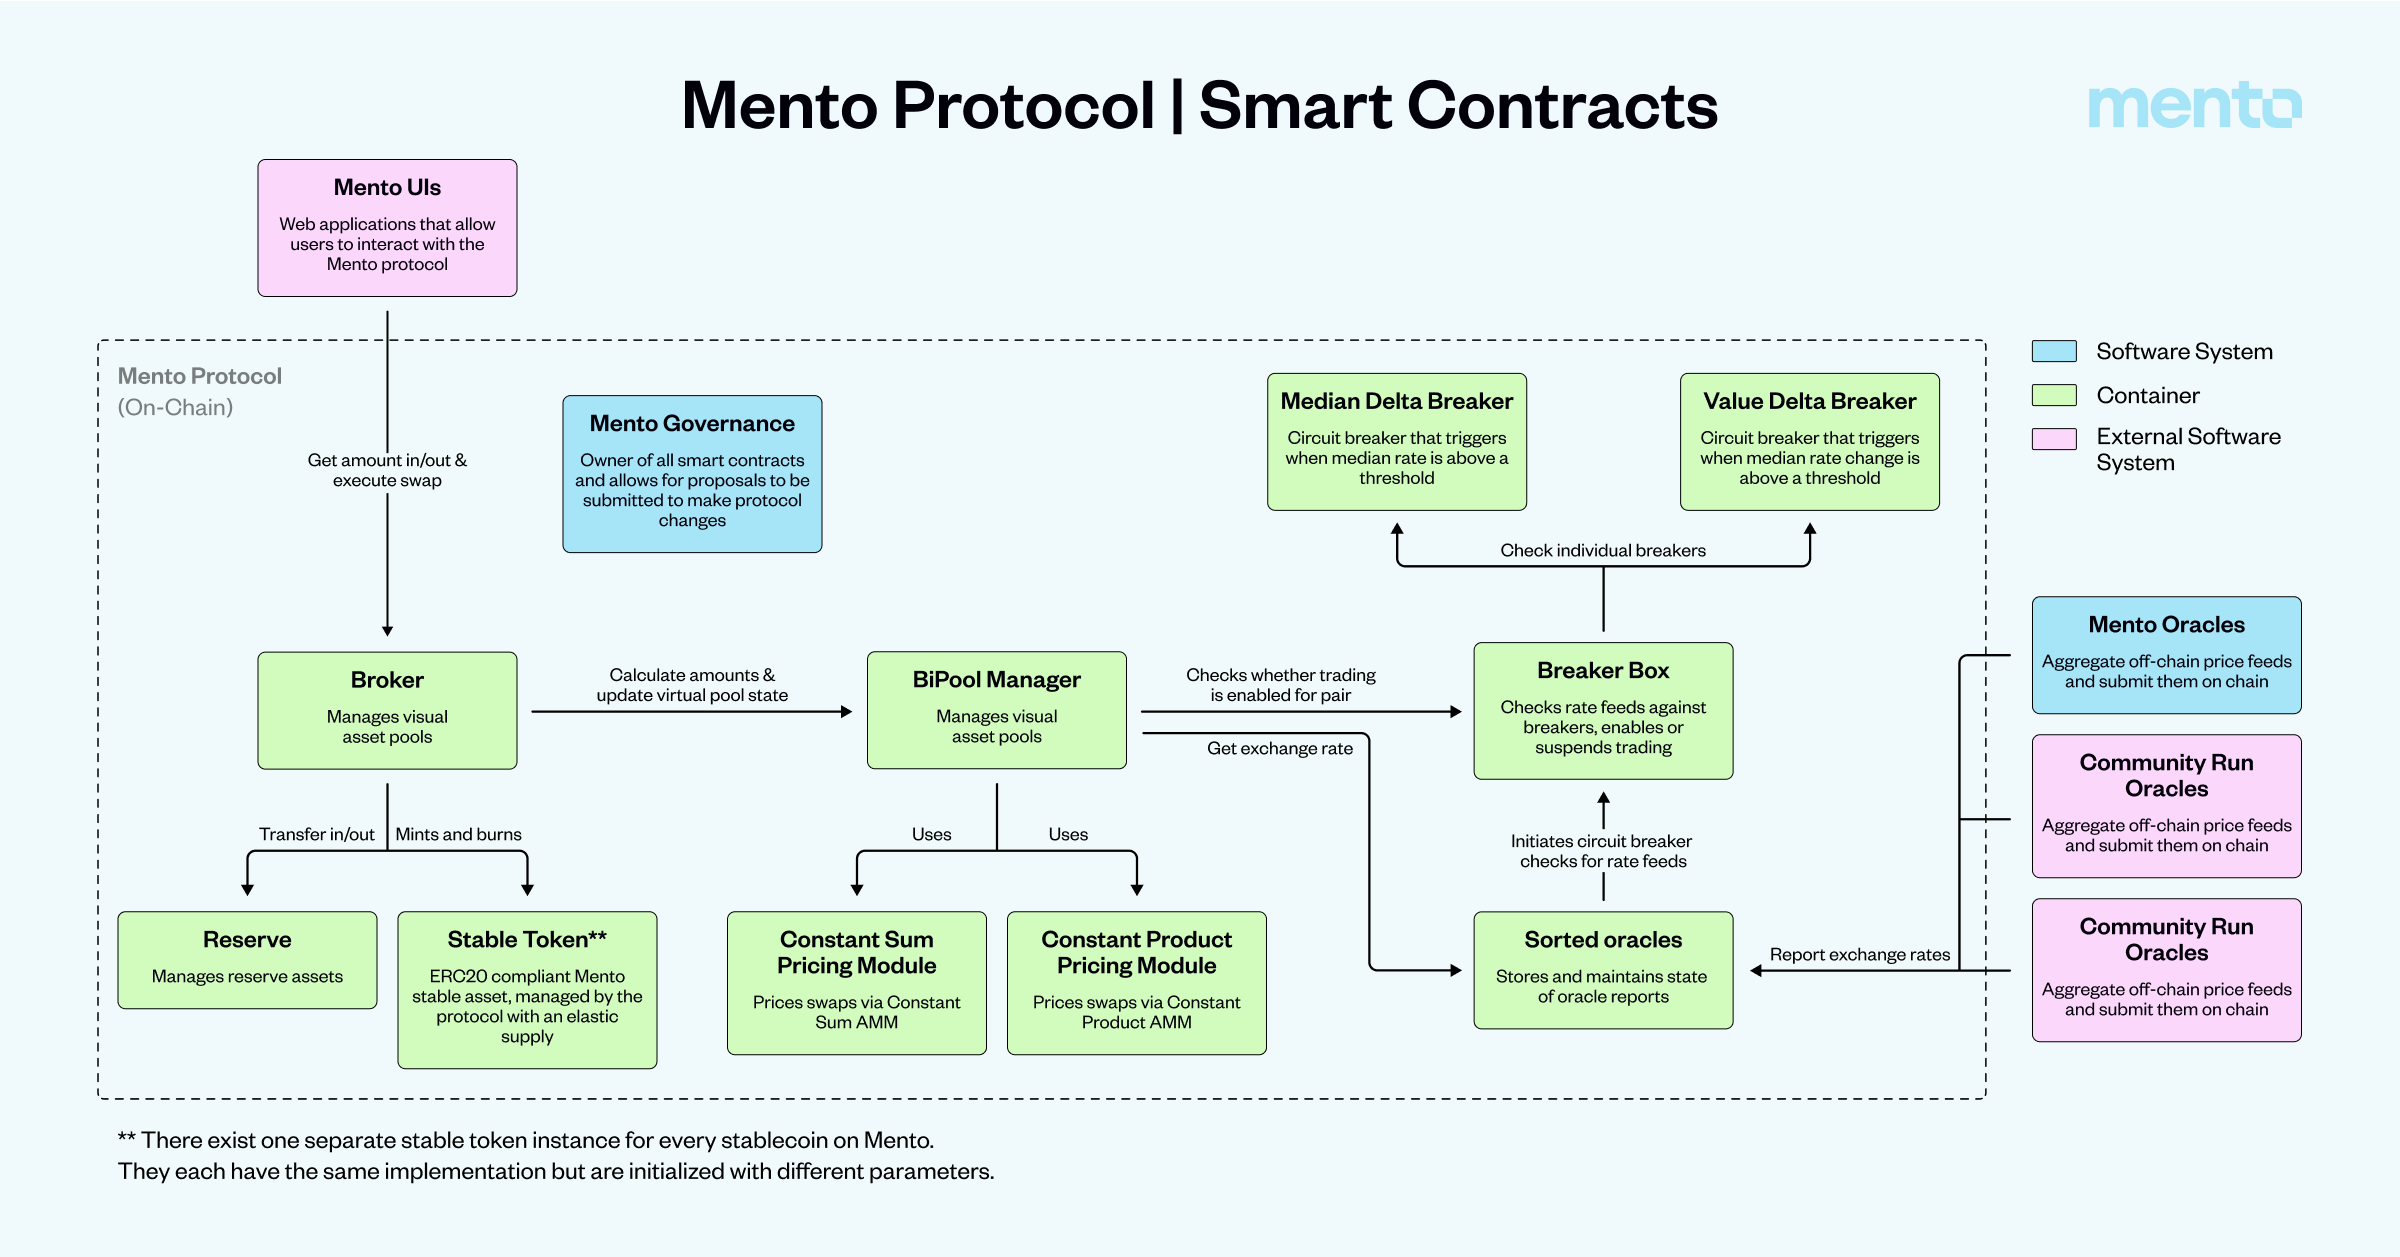
\includegraphics[width=1.0\linewidth]{figures/mento_asset_exchange.png}
    \caption{The Mento Asset Exchange architecture.}
    \label{fig:mento_asset_exchange}
\end{figure}

The following subsections explain the main components of the Mento Asset Exchange Protocol, the Broker, the Exchange Providers and the On-Chain Circuit Breaker, in more detail.

\subsubsection{The Mento Broker Contract}

The Broker contract is the entry point for interacting with the asset exchange protocol. It fulfills three main responsibilities:

\begin{itemize}
    \item Discoverability: It maintains a comprehensive list of all exchange providers registered in the system.
    \item Treasury Management: It has spending rights on the Mento Reserve and can mint and burn any stable asset in the system, thus it is responsible for moving assets during a trade.
    \item Safety and Security: In service of stability, it enforces trading limits in the protocol, constraining the volume of assets that can be traded over time.
\end{itemize}

It is responsible for managing Mento Reserve assets and is the only smart contract with spender rights of the Reserve as well as minting and burning rights over stable assets.\footnote{For more information on the Mento Reserve, such as current collateral, see \cite{mento_reserve}.} 

When executing swaps, the Broker also enforces trading limits. These limits restrict the volume of assets that can be exchanged within a certain timeframe, promoting a balanced and orderly market. There are two types of limits that can be created:

\begin{itemize}
    \item Time-based Limits: Set for specific intervals, these limits control the amount of a particular asset that can be traded, helping to manage liquidity and market order.
    \item Global Limits: In addition to time-based limits, global trading caps are established to maintain long-term stability and prevent large-scale market manipulation.
\end{itemize}

While the Broker is responsible for moving around assets during a swap, it relies on Exchange Providers like the BiPoolManager for pricing trades.

\subsubsection{Exchange Providers and the BiPoolManager}
The concept of exchange providers allows to remove how asset exchanges are priced from the Broker's responsibilities. Given an in asset and an out asset and the amount one wants to trade, an exchange provider can employ any mechanism in order to price the respective trade and manage its internal state as a result of executing such trades. It does this entirely virtually and never actually holds assets.

The first exchange provider implemented in the Mento Protocol is the BiPoolManager. The BiPoolManager is an exchange provider that manages virtual automated market makers (vAMMs) of a pair of Mento assets, which can be either stable-to-collateral or stable-to-stable. vAMMs are built on the same concepts as AMMs; however, there is no user-provided liquidity, and the vAMM holds no assets. A vAMM on Mento can currently be configured to use either a constant sum or a constant product pricing function via pricing modules. Additional pricing models can be added in a modular way.  

A pricing function is a mathematical formula used by AMMs and vAMMs to determine the price of assets in a pool and to determine the levels of available liquidity. Several pricing functions exist, including constant product, constant sum, and constant mean. Mento pricing modules are an abstraction over these pricing functions, allowing Mento exchanges to use any pricing function without changing the underlying code structure.

\subsubsection{On-ChainCircuit Breaker and the Breaker Box}

The Mento Protocol relies on off-chain oracle clients to provide crucial price data such as exchange rates of a specific token against various currencies such as USD, BRL and EUR. These rates are submitted to a smart contract called SortedOracles. The protocol includes an on-chain circuit breaker as an additional security measure to protect the protocol against manipulation of the submitted rates as well as extreme volatility during black-swan type market conditions.

The circuit breaker pattern is typically used in software to prevent catastrophic cascading failures across related systems. This pattern is also adopted in traditional financial markets to trigger a temporary halt in trading when a significant price movement occurs. In the context of Mento, the circuit breaker can be described as a mechanism designed to automatically halt the ability to exchange Mento assets due to a predefined condition being met. The use of the circuit breaker is an attempt to balance the need for market efficiency with the need to prevent catastrophic losses due to extreme circumstances.

Mento's on-chain circuit breaker is not a single component but a collection of components designed to identify specific market conditions and prevent further minting or burning of Mento stables if any of these conditions are met. It was built with flexibility in mind and allows the monitoring of new conditions and the integration of additional virtual asset pools in the future. Figure \ref{fig:circuit_breaker} gives an overview over the circuit breaker architecture.

\begin{figure}[ht]
    \centering
    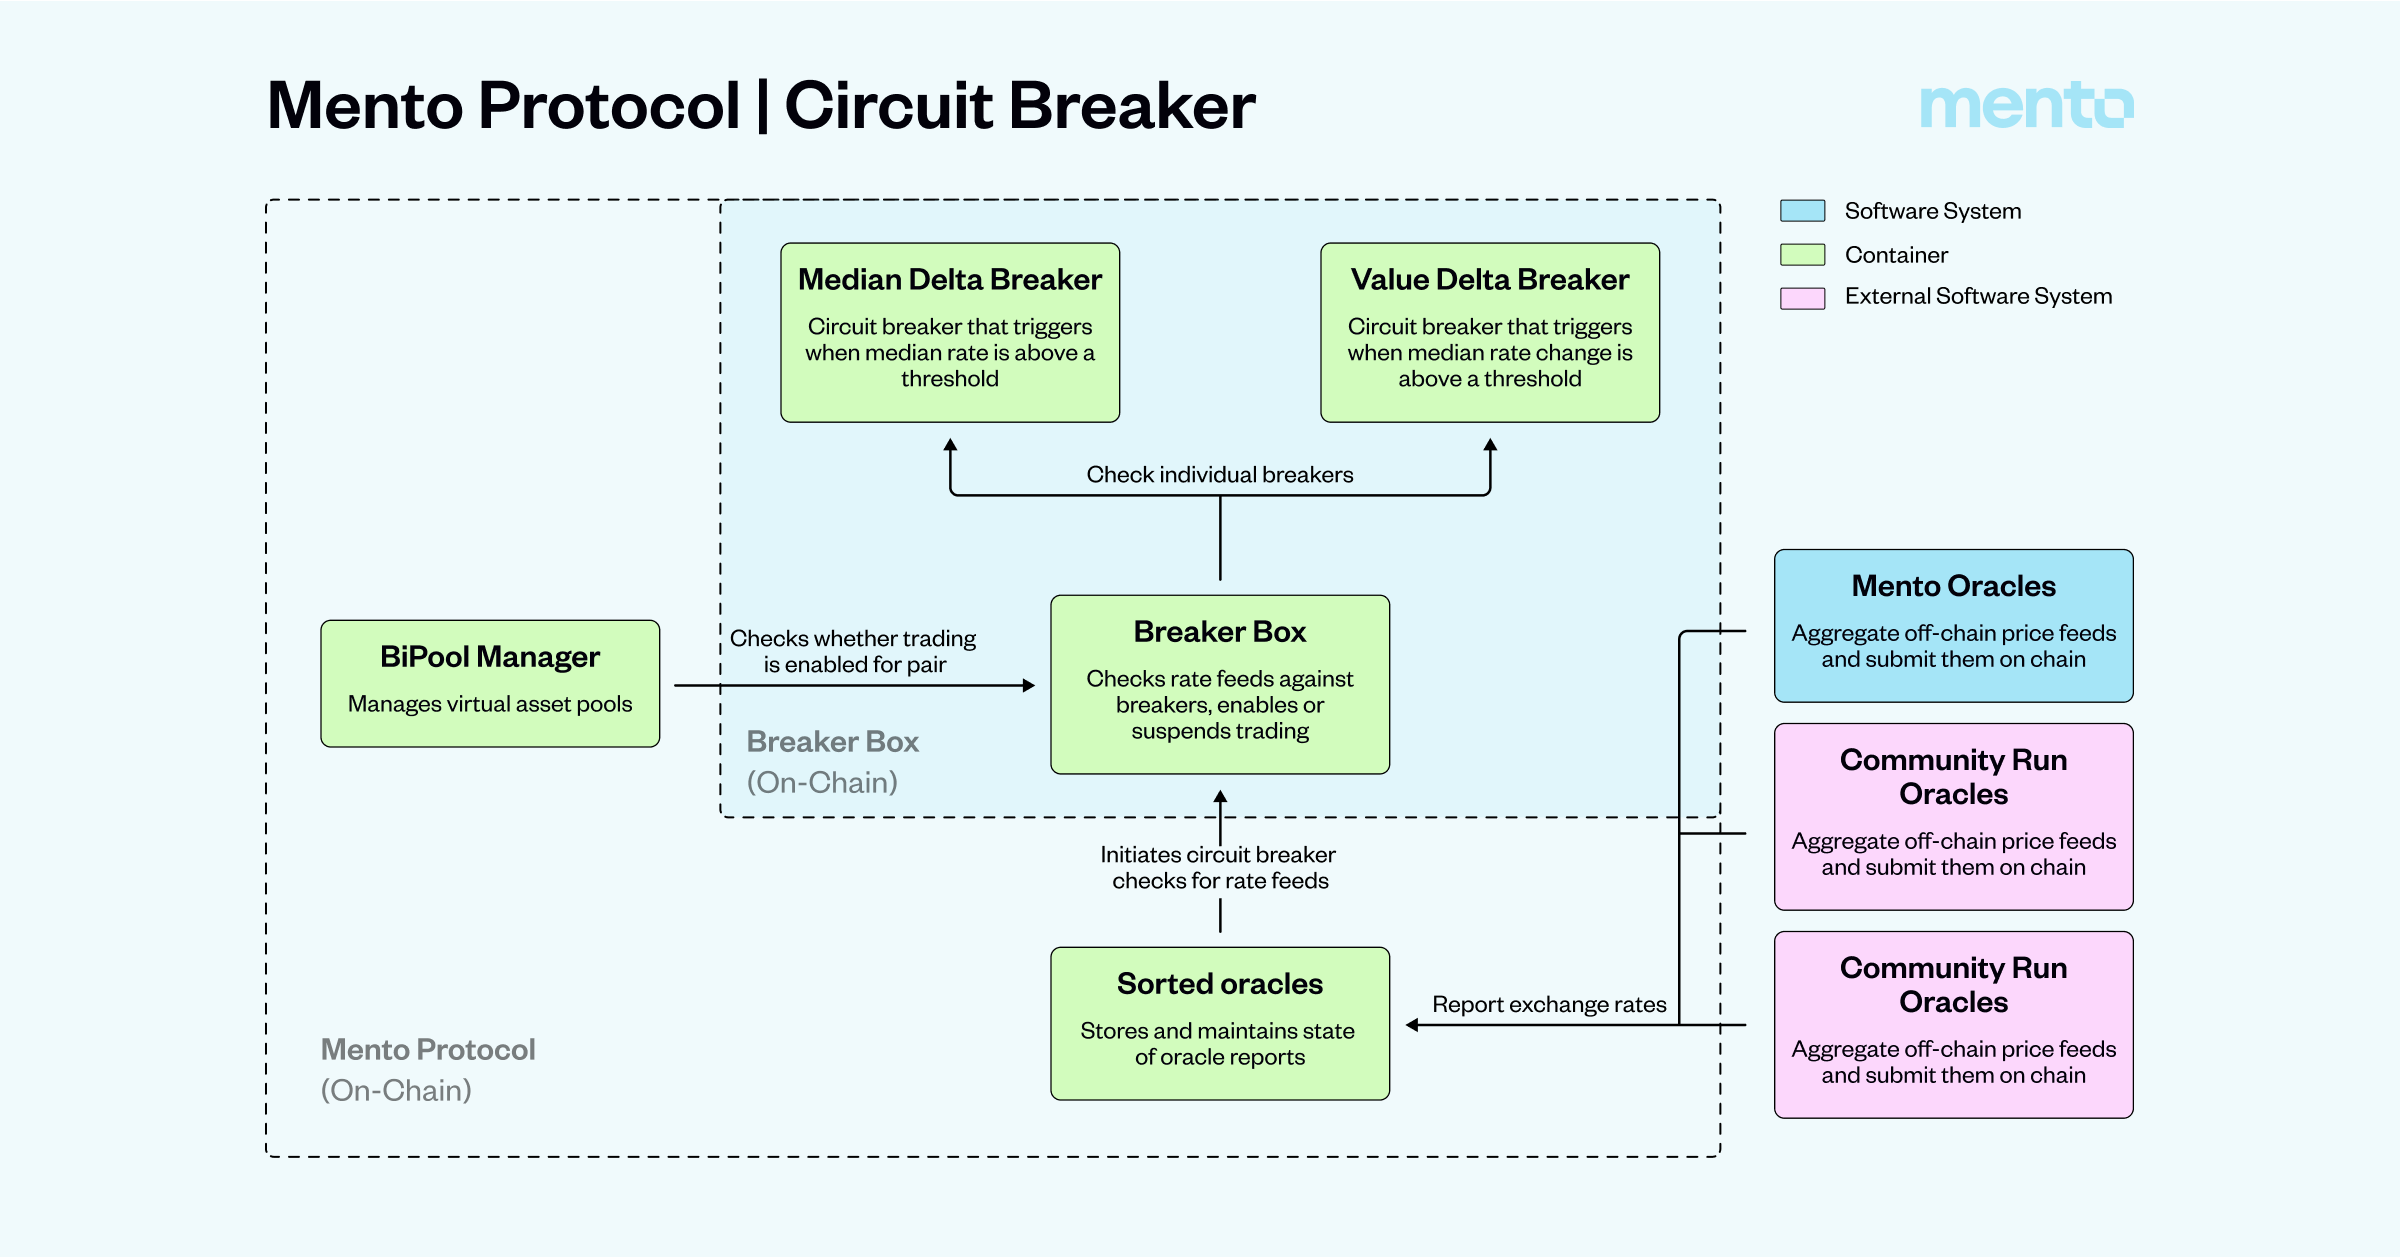
\includegraphics[width=1.0\linewidth]{figures/mento_circuit_breaker.png}
    \caption{The Mento Circuit Breaker Architecture}
    \label{fig:circuit_breaker}
\end{figure}


\subsection{Mento Stablecoin Factory}

The vision of the Mento Platform extends beyond mere stability; it encompasses the creation of a diverse array of decentralized stablecoins tailored to specific use cases by a variety of operators. To realize this vision, Mento must provide a robust toolkit offering the core functions necessary to swiftly deploy new decentralized stablecoins at scale while ensuring the integrity of products launched on the platform. This section introduces the Stablecoin Factory, an essential addition to the Mento Platform, designed to fulfill this need.

Currently, the process of launching new assets on Mento demands significant engineering effort and specialized domain knowledge from the team. However, this approach lacks scalability, as it results in a linear dependency between the number of assets launched and the available engineering capacity over time. To address the growing demand for multiple decentralized stablecoins with diverse designs, automation of the launch process becomes imperative.

The Stablecoin Factory represents a no-code toolkit for launching new assets in a permissionless and decentralized manner. It streamlines the deployment process, allowing operators to initiate the creation of a new stablecoin by simply invoking a function of a smart contract and providing the necessary parameters, such as reference price feed, collateral asset, and token name/ticker. Upon selection, the Stablecoin Factory deploys a suite of smart contracts constituting a functional decentralized stablecoin, including an ERC-20 token contract, a Vault Factory for borrower interactions, and a Stability Pool for funding liquidations when required. Figure \ref{fig:stablecoin_factory} illustrates the high-level architecture of the Mento Stablecoin Factory. 

\begin{figure}[ht]
    \centering
    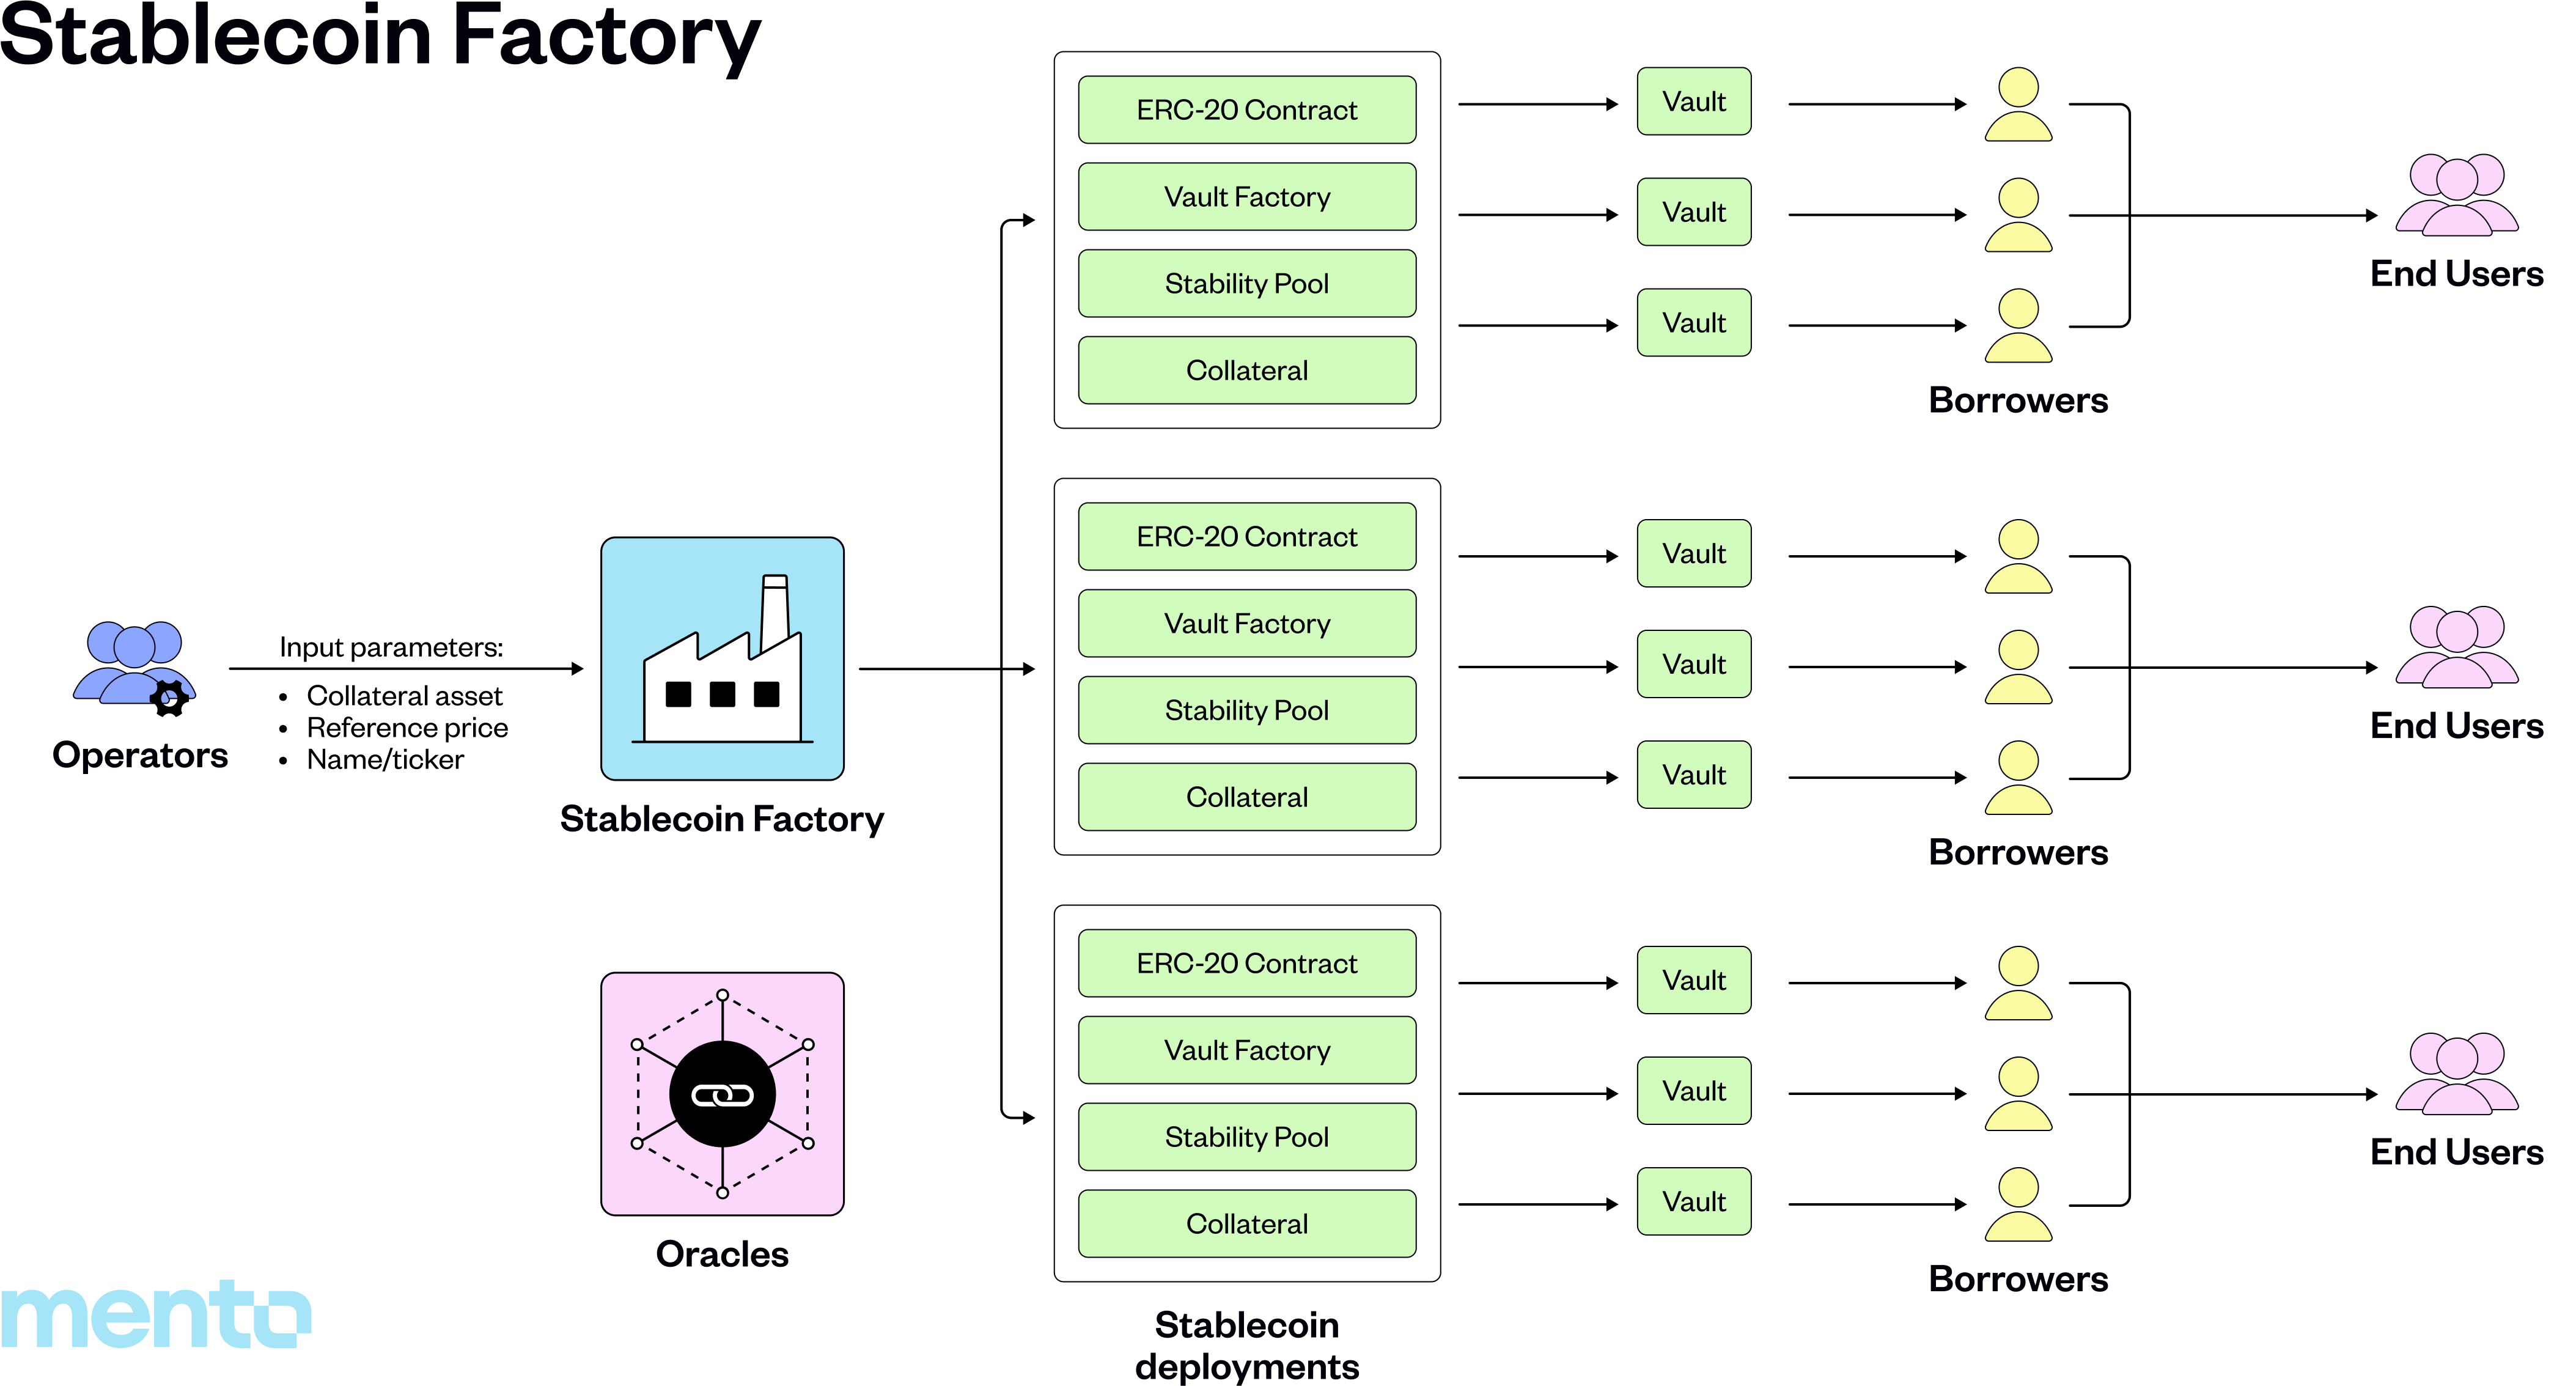
\includegraphics[width=1\linewidth]{figures/stablecoin_factory.png}
    \caption{This figure provides an overview over the high-level architecture of Mento's Stablecoin Factory.}
    \label{fig:stablecoin_factory}
\end{figure}

\subsubsection{Core Components}
\begin{itemize}
    \item CDP Module: At the heart of the Stablecoin Factory lies the Collateral Debt Position (CDP) Module, facilitating the borrowing of decentralized stablecoins into existence by providing underlying collateral. Particularly suited for assets whose prices exhibit loose correlation with the price of the collateral, the CDP Module transfers currency exchange rate risks from end-users to protocol borrowers. Borrowers must maintain the collateralization ratio (CR) above a certain threshold to prevent liquidation of their collateral, which would be distributed to users providing stablecoins to the Stability Pool.
    \item Oracle Integration: While the current, in-house oracle implementation on Mento provides robust on-chain price feeds for select stablecoins, it may not scale sufficiently to support arbitrary price feeds envisioned by future operators. To overcome this limitation, Mento will integrate with RedStone, tapping into its decentralized network of data providers. RedStone currently offers data feeds for over 1,000 assets, including numerous fiat currencies, with the ability to expand its coverage as needed.
\end{itemize}

\subsubsection{Challenges}
\begin{itemize}
    \item Fragmented Liquidity: The ease and affordability of launching new decentralized stablecoins pose challenges, such as the potential for multiple parties to introduce multiple versions of the same asset, leading to fragmented liquidity. To mitigate this, Mento will implement an incentivization module, enabling operators and users to incentivize borrowers and liquidity providers. Through the Gauge System, holders of MENTO governance tokens can direct a portion of future token emissions to specific asset stability pools or liquidity pools, fostering liquidity for meaningful assets while rendering less favored 
    assets irrelevant.
    \item Safeguarding Users: Ensuring end-user protection against stablecoins launched with questionable economic setups or malicious intent is paramount. While operators have the flexibility to select any collateral asset, the requirement of a price feed from data providers like RedStone limits the assets eligible for use as collateral. Additionally, the Gauge System acts as a second line of defense, allowing the community to review and reject assets lacking sound economic fundamentals through governance decisions.
    \item Governance and Revenue Sharing: The fee income generated by the Stablecoin Factory is expected to be allocated between the Mento treasury, Mento contributors and MENTO token holders participating in the governance process. Token holders can vote on specific stablecoin pools, ensuring community involvement in decision-making processes.
\end{itemize}

\subsection{ MENTO Governance Token}
The MENTO token is powering a governance framework that emphasizes inclusivity, sustainability, and decentralization. The MENTO token allows stakeholders to engage actively in the platform's development and decision-making processes. Additionally, it facilitates the capture and distribution of platform utility, ensuring that value generated within the ecosystem is shared among participants and contributors in a fair and equitable manner. The following section provides an overview over the main building blocks behind the MENTO token and the on-chain governance infrastructure.

\subsubsection{Core Components}
\begin{figure}[ht]
    \centering
    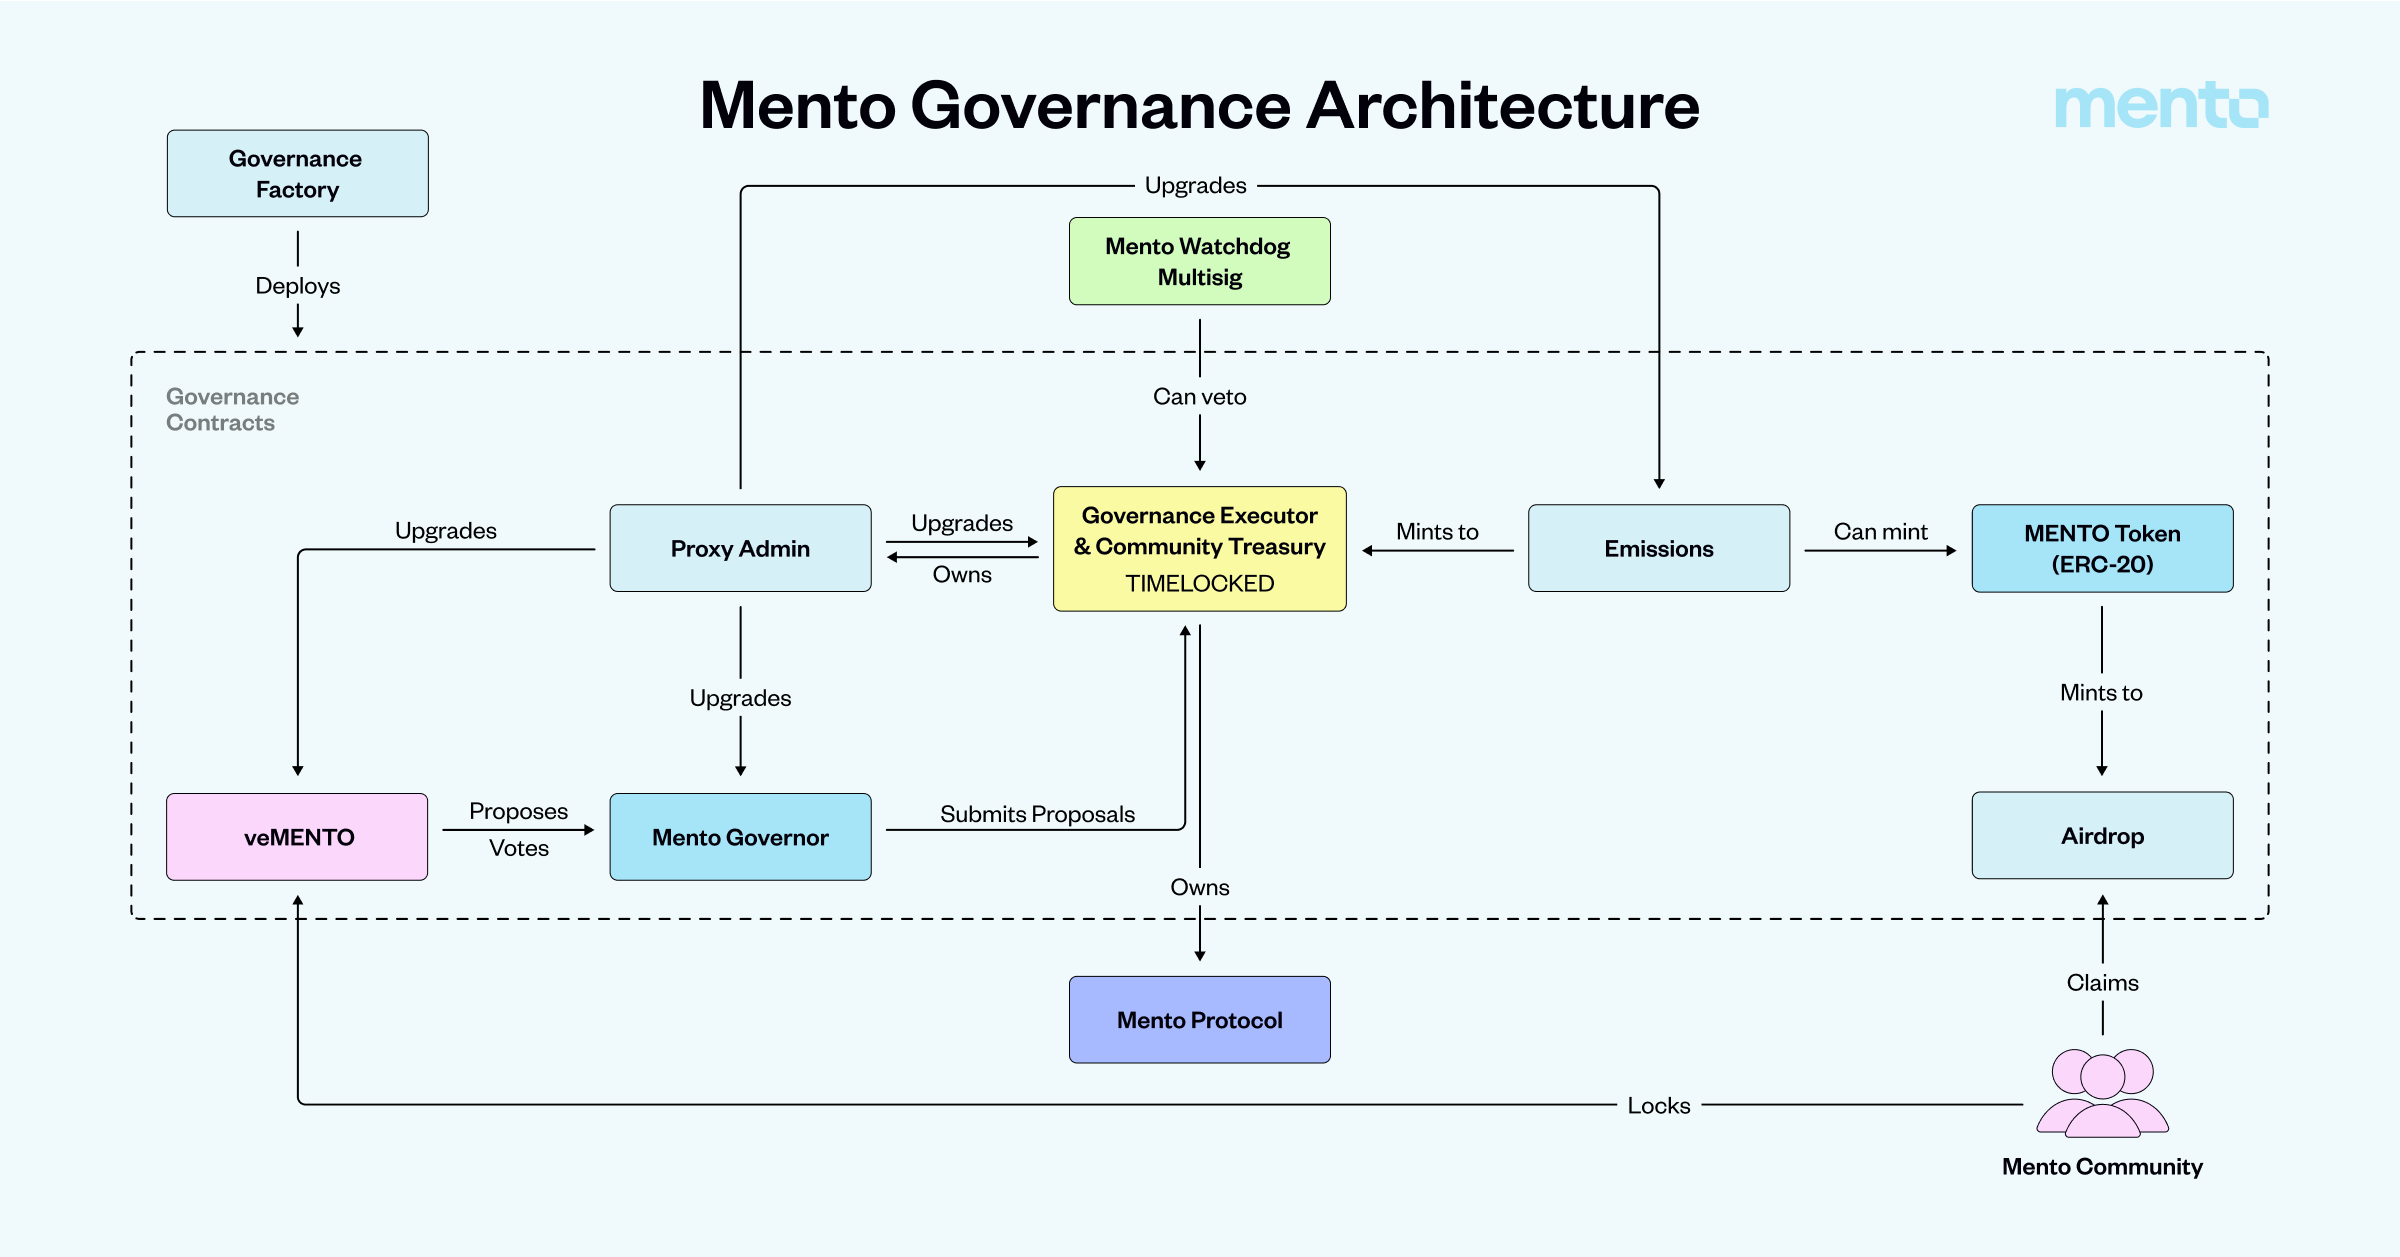
\includegraphics[width=1\linewidth]{figures/mento_governance.png}
    \caption{This figure illustrates the architecture of Mento Governance.}
    \label{fig:mento_governance}
\end{figure}
In addition to the MENTO token, the Mento Protocol introduces veMENTO (vote-escrowed MENTO), a locked version of the token that empowers holders to actively participate in the governance process. The veMENTO concept draws inspiration from the veModel, an on-chain governance framework pioneered by Curve Finance and embraced by various protocols within the ecosystem.

veMENTO holders demonstrate a long-term commitment to the protocol by locking their tokens for varying durations, ranging from one week to four years. This mechanism incentivizes sustained engagement and rewards individuals who contribute to the protocol's long-term success. Through veMENTO, holders accrue enhanced voting power commensurate with the duration of their lock-up period, amplifying their influence in shaping governance decisions and fostering a vibrant and resilient ecosystem.

Key smart contract components of Mento governance are illustrated in Figure \ref{fig:mento_governance} and include:
\begin{itemize}
    \item ERC-20 Smart Contract: The MENTO token functions as an ERC-20 standard token, facilitating seamless integration with decentralized applications and exchanges.
    \item Voting Escrow: A staking contract allows users to lock MENTO tokens in exchange for veMENTO tokens which represent governance rights, encouraging active participation and rewarding long-term commitment.
    \item Governor Contracts: On-chain governance contracts oversee smart contracts, treasury management, reserve allocation, and protocol adjustments in a decentralized manner.
    \item Emission Contract: Controls the issuance of MENTO tokens to the treasury, regulating protocol spending and ensuring sustainable growth.
    \item Community Treasury: Receives emissions from MENTO tokens, enabling governance to allocate resources efficiently and support platform initiatives.
    \item Watchdog Multisig: In general terms, a "watchdog" refers to an individual or group that monitors the activities of another entity (such as an individual, corporation, non-profit group, DAO, community, or governmental organization) on behalf of the public to ensure that the entity behaves according to its set purpose and does not act illegally or unethically. In the case of the Mento Protocol, in particular, a watchdog means a group of individuals who will oversee the protocol's governance process, making sure that the technical part of the governance proposals (execution code) exactly matches what's written in the proposal itself. Initially, it is a 3 out of 9 SAFE multi-signature wallet (multisig) with a special right to veto (meaning to cancel the execution of) any governance proposal within 48 hours after it passes.
\end{itemize}

\subsubsection{Tokenomics and Distribution}
At the genesis block (the block at which the MENTO token and governance are deployed), the MENTO token will be non-transferable. Holders can claim their allocation, locked as veMENTO, and participate in governance, but not transfer tokens. At some point in the future, when certain milestones decided by the community have been reached, the transferability of the token will be enabled. At that point in time, it should be possible to sell/buy the token on a secondary market and freely transfer it. The enabling of transferability is subject to on-chain governance.

The allocation plan for the MENTO token was developed to embody fairness, foster community engagement, and ensure the ecosystem's sustainability. The initial token supply allocation contains a notable 45\% designated to the Mento Community Treasury. This allocation is pivotal for providing sufficient resources for the platform's continuous development, the advancement of community-centric initiatives, and the broad growth of the ecosystem.

The MENTO token will have a maximum total supply of 1,000,000,000 (one billion) tokens (also referred to as fully diluted supply going forward). Figure \ref{fig:mento_distribution} provides a high-level overview over the initial distribution. More detail on each individual distribution is provided thereafter.

\begin{figure}[ht]
    \centering
    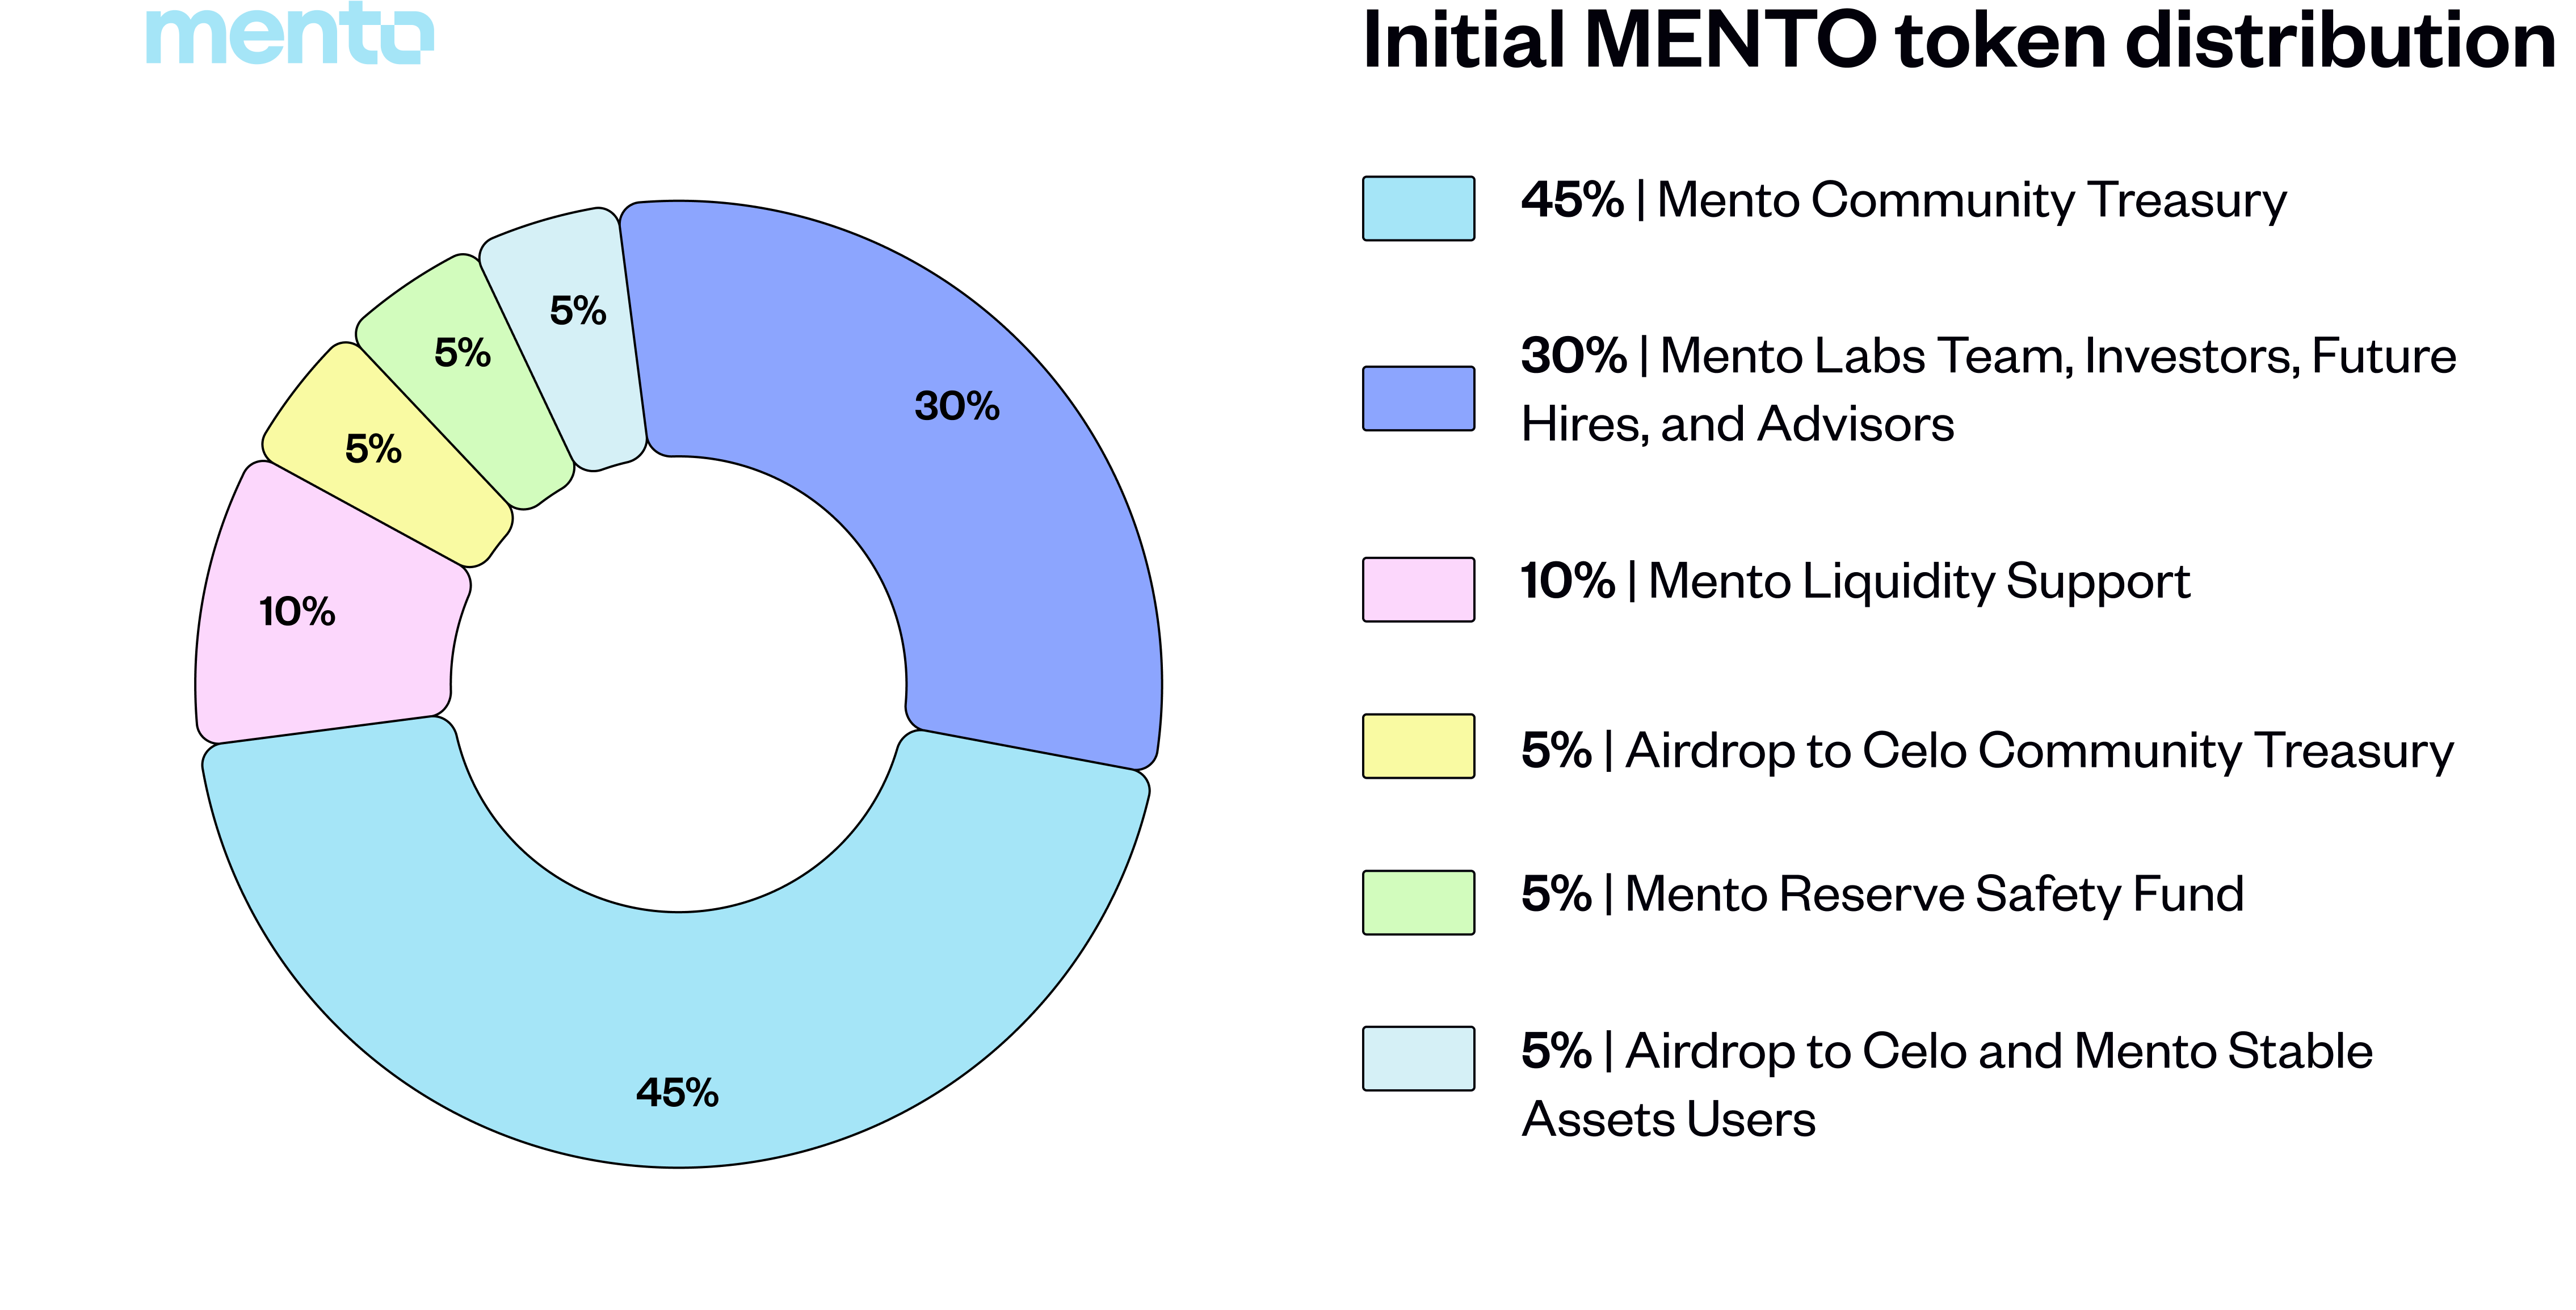
\includegraphics[width=1\linewidth]{figures/mento_distributions.png}
    \caption{MENTO token allocation.}
    \label{fig:mento_distribution}
\end{figure}

\subsubsection*{Mento Community Treasury}
\begin{itemize}
    \item Purpose: The Mento community can spend tokens from the treasury to foster the platform's development. The tokens can be spent on grants, liquidity incentivization programs, etc. The decision to spend tokens from the Treasury is always subject to governance.
    \item Distribution: 450M tokens (45\% of fully diluted supply) with 50M available at genesis block. The tokens will be emitted to the Treasury via exponential decay with a half-life of 10 years. This approach aims to manage the introduction of new tokens into the market gradually and provides an upper bound on spending for the Mento Community Treasury. The emission schedule over time is visualized in Figure \ref{fig:mento_emissions}.
    \item Voting rights: No.
\end{itemize}
\begin{figure}[ht]
    \centering
    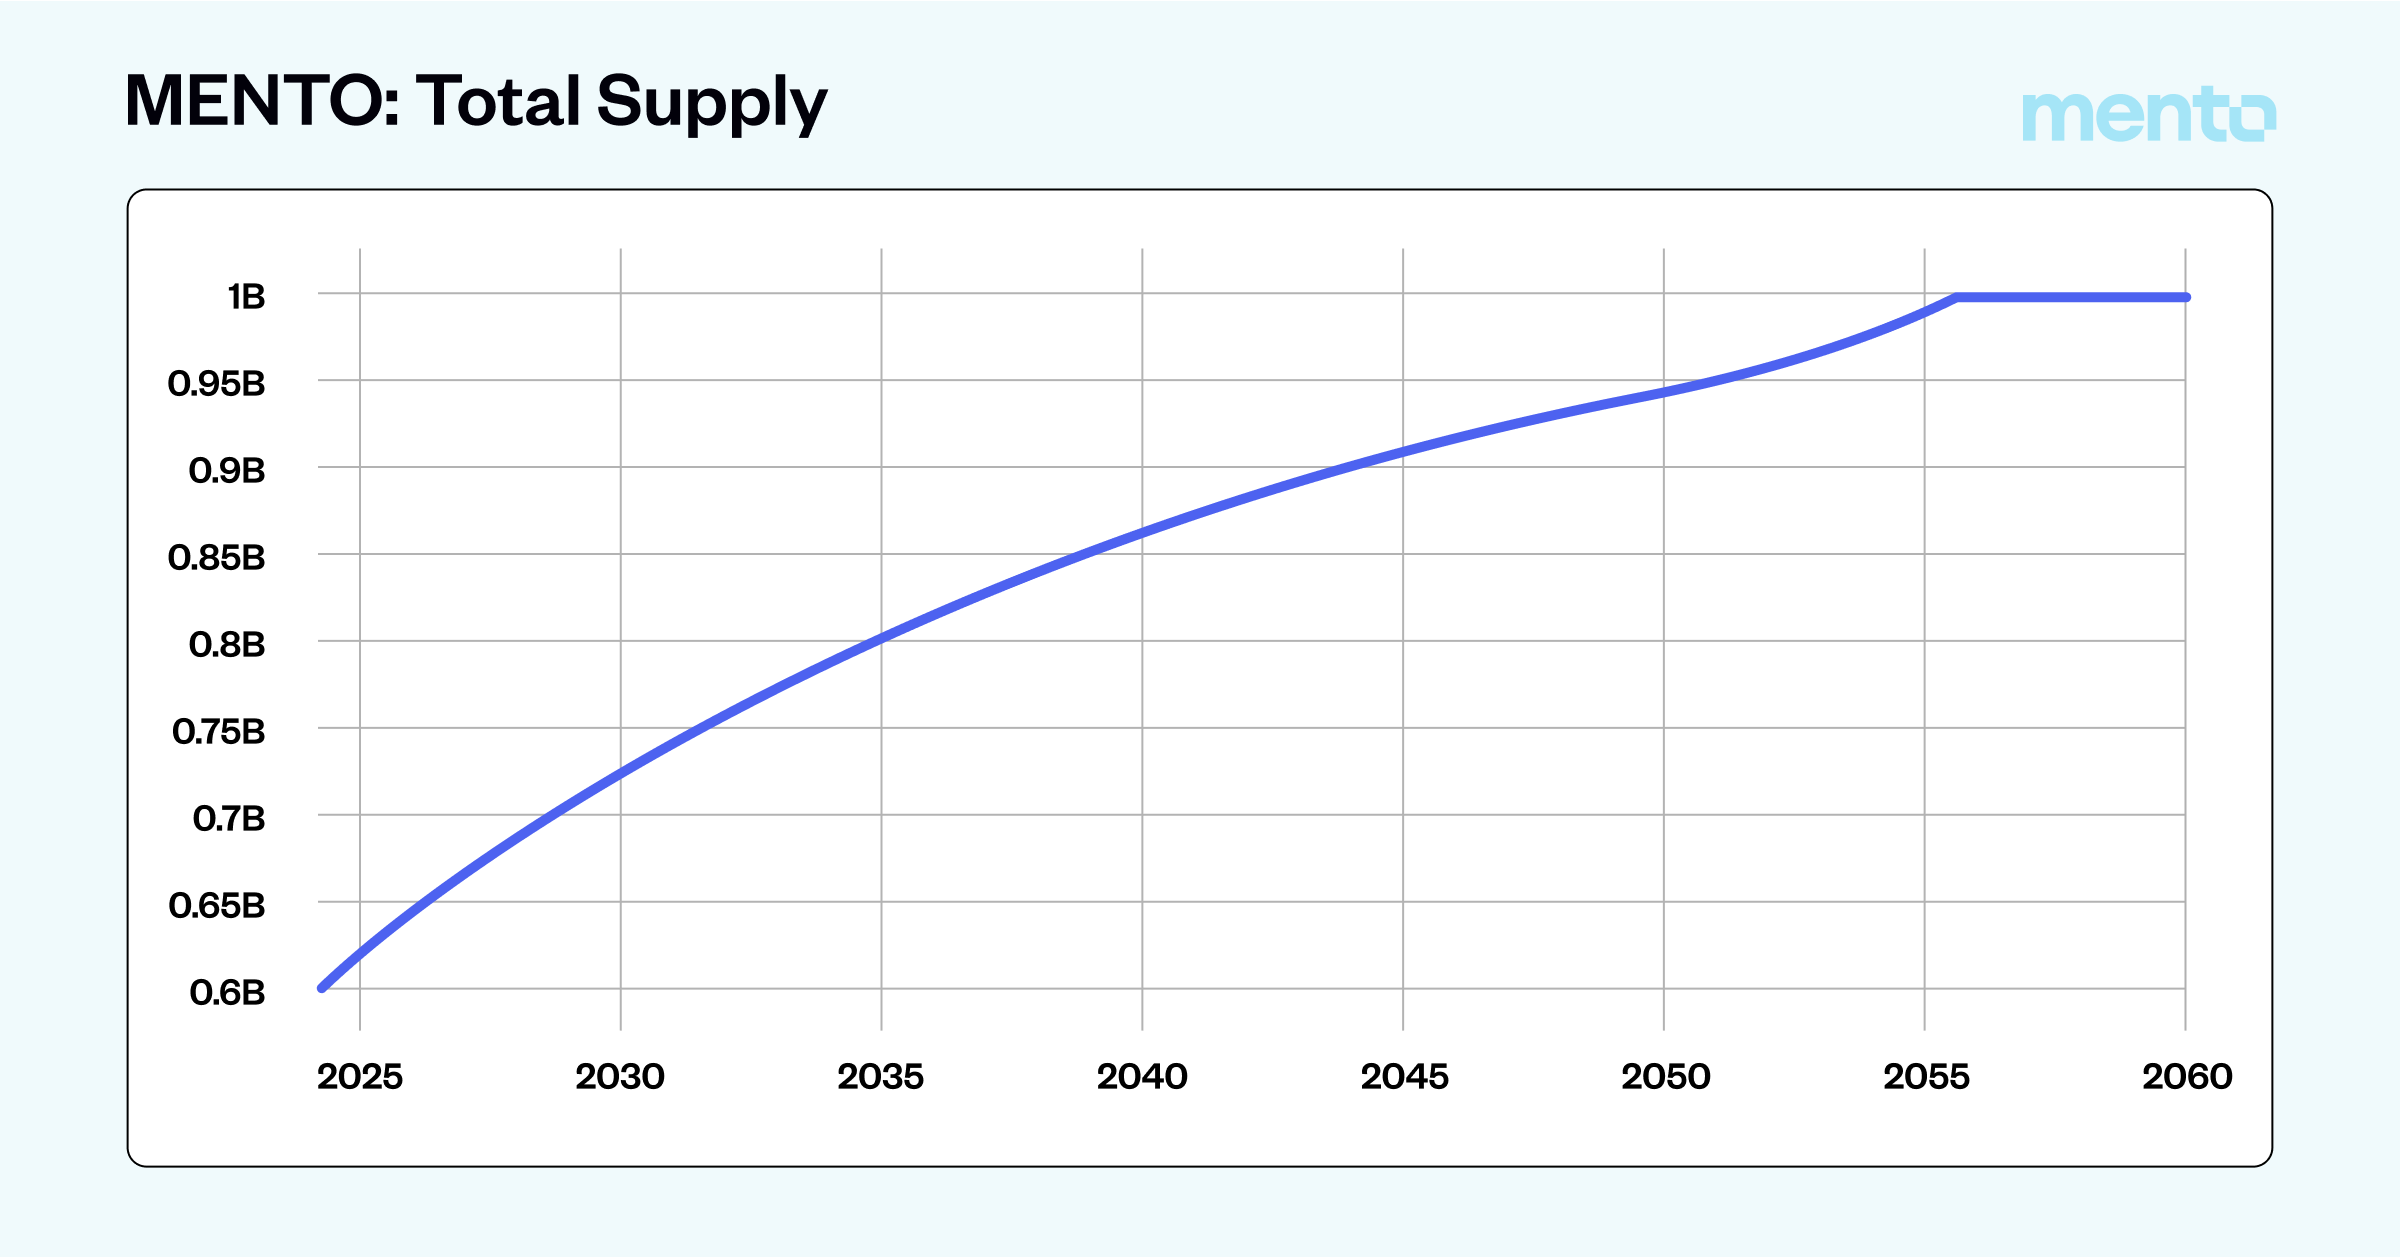
\includegraphics[width=1\linewidth]{figures/mento_emissions.png}
    \caption{MENTO token emissions over time.}
    \label{fig:mento_emissions}
\end{figure}


\subsubsection*{Mento Labs Team, Contributors, Supporters, Future Hires, Advisors}
\begin{itemize}
    \item Purpose: Reward core contributors, supporters, and advisors. Get the best talent to contribute to the protocol in the future.
    \item Distribution: 300M tokens (30\% of fully diluted supply). Existing Mento Labs employees\footnote{For information on Mento Labs, see \cite{mento_labs_website}.}, supporters, and advisors will receive their MENTO tokens split into two parts:
    \begin{itemize}
        \item veMENTO portion (25\% of the allocation):
        To seed voting power to the team and supporters, 25\% of the allocation will be distributed as veMENTO locked for 1 year starting at the token distribution event. The allocation will allow team members to vote from day one using delegation. However, the beneficiary will only get full control of the lock after their cliff period has passed.
        \item MENTO portion (75\% of the allocation): 75\% as MENTO with 1 year delay and 3 years linear vesting starting at the token distribution event via Hedgey token vesting platform. 
    \end{itemize}
    \item Voting rights: Yes, with the veMENTO portion.
\end{itemize}

\subsubsection*{Airdrop to CELO holders and Mento Stable Assets users}
\begin{itemize}
    \item Purpose: Reward existing community members and users for their past contributions to the development and usage of Mento stable assets and the Celo ecosystem overall. 
    \item Distribution: 50M tokens (5\% of fully diluted supply). Owners of eligible addresses can claim their allocation, which they will receive as a veMENTO locked for 2 years with linear unlock. Eligibility criteria apply.
    \item Voting rights: Yes.
\end{itemize}


\subsubsection*{Airdrop to Celo Community Treasury}
\begin{itemize}
    \item Purpose: Long-term incentive alignment between the Celo and Mento communities.
    \item Distribution: 50M (5\% of fully diluted supply) with a 2-year delay followed by a 6-year linear vesting period via the \href{https://hedgey.finance/}{Hedgey} token vesting platform.
    \item Voting rights: No.
\end{itemize}

\subsubsection*{Mento Reserve Safety Fund}
\begin{itemize}
    \item Purpose: An allocation to the Mento Reserve, which will be used as stablecoin collateral in the worst-case scenario of a loss-of-value in primary collateral (USDC, USDT, DAI, …) through credit default events, hacks, etc. 
    \item Distribution: 50M (5\% of fully diluted supply)
    \item Voting rights: No.
\end{itemize}

\subsubsection{Additional Information About the MENTO Token}
\begin{itemize}
    \item \textbf{Classification and Types of Mento Crypto-Assets}\\
    The MENTO token (MENTO) acts as the governance and utility token of the Mento Protocol and is distinct from Mento Stablecoins. It enables holders to participate in the governance process, influencing the Mento ecosystem's development and strategic direction.

    \item \textbf{Technology and Infrastructure Details}\\
    The MENTO token operates on the Celo blockchain, utilizing advanced smart contract architecture for secure and efficient governance actions, token distribution, and seamless integration with DeFi platforms. This framework supports decentralized governance and enhances interoperability across the blockchain ecosystem.

    \item \textbf{Functional Use Cases within the Ecosystem}\\
    MENTO tokens are instrumental in enabling:
    \begin{itemize}
        \item \textit{Governance Participation:} Holders can propose and vote on changes, driving the ecosystem’s evolution in alignment with community interests.
        \item \textit{Incentive Mechanisms:} Influencing incentive structures within the ecosystem to encourage active participation and contribution.
        \item \textit{Ecosystem Development and Funding:} Facilitating ecosystem growth through strategic project funding and partnership support.
        \item \textit{Stakeholder Engagement:} Fostering a deep level of involvement from all ecosystem participants, aligning their interests with the ecosystem's success.
    \end{itemize}
\end{itemize}


\subsubsection{Rights and Obligations}
This section details the rights associated with the MENTO tokens and the encouraged responsibilities of the holders within the Mento ecosystem, ensuring clarity on the governance participation and the potential of revenue sharing based on future governance decisions.

\begin{itemize}
    \item \textbf{Rights Attached to the Crypto-Assets}
    \begin{itemize}
        \item \textit{Governance Participation:} MENTO token holders are welcomed to partake in the governance processes of the Mento ecosystem. This includes the ability to propose, vote, and influence the ecosystem’s strategic directions and priorities, though participation is voluntary and at the holder's discretion.
        
        \item \textit{Input on Ecosystem Development:} Token holders are encouraged to offer suggestions for ecosystem improvements, including new features and optimizations, contributing to the ecosystem's evolution in a collaborative manner.
        
        \item \textit{Potential Revenue Sharing:} The possibility of platform revenue sharing exists, subject to future governance decisions. Token holders may have the opportunity to participate in the ecosystem's success through mechanisms that will be defined and approved by the community governance processes.
        
        \item \textit{Access to Services:} Holding tokens may provide opportunities for access to certain services within the ecosystem at preferential terms, acknowledging the active role of token holders in the ecosystem’s development.
    \end{itemize}
    
    \item \textbf{Holder Obligations}
    \begin{itemize}
        \item \textit{Engagement in Governance:} Token holders are encouraged, though not obligated, to engage in governance processes, contributing to decisions with informed and thoughtful participation to support the ecosystem’s advancement.
        
        \item \textit{Regulatory Awareness:} Holders must be mindful of and adhere to the regulatory requirements applicable in their jurisdictions, including taxation, compliance with securities laws, and AML regulations, to ensure legal and ethical token usage.
        
        \item \textit{Community Conduct:} A commitment to ethical behavior that upholds the ecosystem's values is expected, including respectful interactions within the community and avoidance of any actions that could harm the ecosystem’s integrity or reputation.
        
        \item \textit{Security Best Practices:} While not a mandate, employing robust security measures to safeguard one's tokens is strongly advised, which includes prudent management of private keys and vigilance against security threats.
        
        \item \textit{Staying Informed:} Though voluntary, staying updated on the ecosystem’s developments and actively participating in discussions and votes when possible, enriches the governance process and contributes to the ecosystem's collective wisdom.
    \end{itemize}
\end{itemize}

The relationship between MENTO token holders and the Mento ecosystem is founded on mutual respect and the shared goal of ecosystem prosperity. The outlined rights offer a framework for active and meaningful participation, while the encouraged responsibilities highlight the importance of mindful engagement in fostering a thriving and sustainable community.

\section{Information on the Risks}
\label{sec:risks}
The Mento Protocol is subject to a variety of inherent risks that can impact stakeholders in different ways. These risks, critical to understand for anyone holding MENTO tokens as well as Mento stablecoin holders, arise from a complex interplay of economic factors, technical challenges, regulatory environments, and market dynamics. This section aims to delineate these risks comprehensively, providing MENTO token holders and Mento stablecoin holders with a detailed insight into potential challenges they may face. Economic stability risks, for instance, highlight the vulnerabilities tied to global financial trends and the protocol's mechanisms for maintaining stablecoin pegs. Similarly, technical risks, including smart contract vulnerabilities and operational hazards, underscore the technological complexities of running a decentralized financial platform. Additionally, evolving regulatory landscapes and fluctuating market conditions present ongoing challenges that can affect the usability, legality, and value of Mento assets. By exploring these areas, this section serves to inform and prepare stakeholders for the multifaceted risk environment of the Mento ecosystem, emphasizing the importance of vigilance and informed participation in mitigating these risks.

\subsection{Risks for MENTO Token Holders}

Holding MENTO tokens involves exposure to governance dynamics, market volatility, and the broader success of the Mento Platform. The broad risk categories include:

\begin{itemize}
    \item \textbf{Smart Contract Risks:} MENTO token holders are subject to the risks inherent in the smart contracts governing the tokens themselves, including the mechanisms for governance and revenue sharing. Vulnerabilities in these contracts could lead to direct financial losses for token holders or undermine the integrity of the governance process.
    
    \item \textbf{Operational Risks:} Similar to stablecoin holders, token holders are also affected by operational risks within the Mento ecosystem. Mismanagement of governance processes, errors in token distribution mechanisms, or loss of critical infrastructure can erode trust in the Mento Platform and diminish the value proposition of MENTO tokens.
    
    \item \textbf{Market and Speculative Risks:} MENTO tokens are subject to market forces that can cause price volatility. Speculative trading, market sentiment, and external economic factors can significantly impact token value.
    
    \item \textbf{Revenue Sharing Uncertainties:} The implementation and success of a utility / revenue-sharing model depend on sustained platform growth. Fluctuations in platform revenue, due to competition or decreased usage, could affect the expected benefits from holding MENTO tokens.
    
    \item \textbf{Platform Evolution and Technological Risks:} MENTO tokens are integral to a platform subject to ongoing development and technological advancements. Changes in protocol, smart contract upgrades, or integration challenges with new technologies could introduce vulnerabilities or diminish the token's utility and value.
    
    \item \textbf{Regulatory Landscape:} The evolving regulatory framework for cryptocurrencies and tokens with governance or profit-sharing features presents a significant risk. Legal challenges, financial regulations, or changes in policy affecting crypto-assets/tokens in terms of e.g. trading, or taxation could impact MENTO token holders disproportionately.

    \item \textbf{Crossover Risk from Mento Stablecoins:} Mento stablecoins can have significant crossover effects on the MENTO token. The interconnected nature of these assets within the Mento ecosystem means that issues impacting the stability, liquidity, or regulatory compliance of Mento stablecoins could directly or indirectly influence the perceived value, usability, and regulatory scrutiny of the MENTO token.
\end{itemize}

\subsection{Risks for Mento Stablecoin Holders}
This section will  delve into the risks inherent to Mento stablecoins in the interest of providing a comprehensive risk overview to support informed decision-making. 
Mento stablecoin holders face a range of risks that can impact the stability and usability of these assets. Key risk areas include:

\begin{itemize}
    
    \item \textbf{Reserve Composition and Performance Risks:} The assets comprising the Mento Reserve are pivotal in ensuring the stablecoins' value. However, these reserves are not immune to market dynamics. Adverse movements in the value of reserve assets, whether due to market downturns or changes in asset-specific fundamentals, pose a risk to the stablecoin's backing. Moreover, the liquidity of these assets is crucial, especially in scenarios requiring quick liquidation to support stablecoin redemptions.

    \item \textbf{Smart Contract Risks:} Both stablecoin and token operations within the Mento ecosystem rely on complex smart contracts. These contracts, while audited, are not immune to vulnerabilities or bugs that hackers could exploit, leading to loss of funds or operational failures. Historical precedents in the broader DeFi space highlight the potential financial and reputational damages from such incidents.
    
    \item \textbf{Operational Risks:} The management of Reserve collateral is a critical operation within the Mento ecosystem. Operational failures, such as incorrect transfer or loss of reserve assets due to human error or system flaws, could significantly impact the Reserve's ability to support stablecoin value. This category of risk also covers failures in executing protocol upgrades or maintaining critical infrastructure.

    \item \textbf{Oracle System Reliability:} Accurate and timely data from oracles are crucial for the protocol's operation, especially in adjusting the supply of stablecoins to match demand and maintain pegs. However, the oracle system faces its own set of challenges, including data manipulation, single points of failure among data providers, and latency in data transmission, all of which could lead to inaccurate adjustments and potential instability.

    \item \textbf{Macroeconomic Risks:} 
    The stability of Mento's stablecoins hinges on a careful balance between supply and demand, supported by the robustness of the Reserve and the adaptability to market dynamics. This equilibrium, however, is vulnerable to a range of macroeconomic disruptions:
    
    \begin{itemize}
        \item \textbf{Market Volatility:} The cryptocurrency market, known for its high volatility, alongside fluctuations in global financial markets, can precipitate abrupt changes in the demand for stablecoins. Such volatility tests the Mento protocol's capacity to rapidly adapt the supply of stablecoins to ensure their pegs remain intact. The agility of this response mechanism is crucial in mitigating the impact of market shocks and preserving the stability of the stablecoins.
    
        \item \textbf{Fiat Currency Instabilities:} The pegging of Mento stablecoins to fiat currencies introduces exposure to the economic health and policies affecting those currencies. Instabilities such as inflation, deflation, or sudden policy shifts (like demonetization or capital controls) in the fiat systems can indirectly compromise the perceived stability and reliability of the stablecoins. These instabilities necessitate continuous monitoring and potentially swift adjustments in the protocol's operations to align with evolving fiat currency landscapes.
    
        \item \textbf{Systemic Financial Crises:} Global or regional financial crises pose systemic risks that can extend to the cryptocurrency space, including Mento's stablecoins. Such crises often result in widespread panic selling, liquidity crunches, and the collapse of financial institutions, challenging the protocol to manage extreme market conditions effectively. The resilience of the Mento ecosystem in such scenarios depends on the strength of its reserve assets and the strategic measures in place to navigate financial tumult.
    
        \item \textbf{Speculative Attacks:} Speculative attacks specifically target the mechanisms maintaining the stablecoin pegs, with attackers aiming to profit from induced instability. These attacks might exploit identified or hypothetical vulnerabilities in the protocol's design or capitalize on broader market insecurities. Defending against such attacks requires not only robust protocol design and security measures, but also a proactive stance in monitoring market activities and potential threats.
    
        \item \textbf{Global Economic Policy Changes:} Shifts in global economic policies, such as changes in interest rates by major central banks, trade policies, or significant economic sanctions, can have far-reaching effects on currency values and financial markets. Such changes can alter the demand for stablecoins as users seek to hedge against uncertainty in traditional financial systems or capitalize on arbitrage opportunities. The protocol must remain flexible and responsive to global economic trends to maintain stablecoin stability in the face of shifting economic policies.
        \end{itemize}
    
        \item \textbf{Regulatory and Compliance Risks:} The regulatory landscape for cryptocurrencies and stablecoins is evolving. New regulations, or changes to existing ones, could impact the operation, legality, and fiscal treatment of Mento stablecoins across different jurisdictions. Such changes could alter the risk profile of holding or using stablecoins, affecting their demand and stability.
    
        \item \textbf{Adoption and Ecosystem Risks:} The value proposition of Mento stablecoins is also tied to their integration within the cryptocurrency ecosystem. Challenges in achieving widespread adoption, whether due to competitive pressures, technical barriers, or shifts in market preferences, can limit their utility and, by extension, their demand and stability.
    
    \end{itemize}

Hence, both, MENTO token holders and Mento stablecoin holders, navigate a landscape filled with diverse and evolving risks. For stablecoin holders, the emphasis is on the stability and usability of their assets amidst economic fluctuations and regulatory changes. For token holders, the concerns broaden to include governance dynamics, market volatility, and the long-term success and adaptability of the Mento Platform. Stakeholders are encouraged to remain informed and actively engaged in the community to navigate these risks effectively.

\subsection{Risk Acknowledgement}
This whitepaper explicitly acknowledges the following concrete risks for holders of the MENTO token as well as holders of Mento stablecoins:

\begin{itemize}
    \item \textbf{Potential Loss of Value:} The value of the MENTO token and Mento stablecoins is subject to market volatility and can decrease, potentially resulting in partial or complete loss of investment. Factors influencing this risk include market trends, regulatory developments, and changes in technology.
    
    \item \textbf{Transferability Restrictions:} There might be conditions under which the MENTO token and Mento stablecoins cannot be freely transferred. Such limitations could arise from regulatory decisions, platform-specific rules, or network issues, potentially affecting the ability to trade or move the token.
    
    \item \textbf{Liquidity Constraints:} The liquidity of the MENTO token and Mento stablecoins - its ease of conversion into fiat or other cryptocurrencies without substantial loss - is not guaranteed. Market fluctuations, trade volumes, and participant activities could impact the token's liquidity, possibly restricting sales at desired prices.
    
    \item \textbf{Exclusion from Investor Compensation Schemes:} Stakeholders should be aware that the MENTO token and Mento stablecoins do not qualify for investor compensation schemes. These protections, common for traditional financial instruments, do not apply to losses incurred from the MENTO token or Mento stablecoins.
    
    \item \textbf{Exclusion from Deposit Guarantee Schemes:} Similarly, the MENTO token and Mento stablecoins are not covered by deposit guarantee schemes, which protect bank deposits against bank failures. This level of protection is not available for holders of the MENTO token or holders of Mento stablecoins.
\end{itemize}

This description and acknowledgment of risks associated with the MENTO token as well as Mento stablecoins is intended to equip stakeholders with a clear understanding of the potential challenges ahead. Stakeholders are encouraged to undertake comprehensive due diligence and evaluate their financial condition and risk appetite before engaging with the MENTO token and Mento stablecoins.

\section{Roadmap and Future Developments}
\label{sec:roadmap}

The Mento Platform's development path is structured around clear, actionable objectives aimed at broadening its financial ecosystem. Central to this expansion are the introduction of the MENTO token, the establishment of a decentralized governance structure, and the activation of the Stablecoin Factory.

\begin{itemize}
    \item \textbf{Deployment of the Stablecoin Factory:}
    Planned to launch during Q2/2024, the Stablecoin Factory is a pivotal innovation designed to facilitate the easy creation and launch of new stablecoins. This toolkit allows for the rapid deployment of assets pegged to a diverse array of fiat currencies, commodities and more, significantly broadening the platform's utility and reach. The first phase will see the introduction of stablecoins tied to key emerging market currencies, addressing the demand for digital assets in economies currently underserved by the current US-Dollar focused stablecoin solutions available.

    \item \textbf{Launch of the MENTO token:}
    The launch of the MENTO token is planned for Q2/2024. MENTO will serve as the cornerstone of the platform's governance model, enabling token holders to vote on key proposals and influence the platform's direction. The token launch is a critical step towards decentralizing decision-making processes and aligning the platform's development with the community's needs and values. It will also allow for incentivizing certain behavior on the platform and directing and sharing platform revenue.

    \item \textbf{Initiation of Mento Governance:}
    Coinciding with the MENTO launch, the platform will transition to a decentralized governance framework. This new structure will empower the community to propose, debate, and implement changes directly through a democratic voting process. Initial governance actions will likely focus on bootstrapping and launching the Stablecoin Factory, setting the stage for community-led development and innovation.

    \item \textbf{Integration and Partnership Enhancements:}
    Beyond internal developments, the roadmap includes strategic partnerships aimed at enhancing platform interoperability and user access. These collaborations will extend the reach of Mento's stablecoins and the MENTO token across various wallets, exchanges, and DeFi platforms, ensuring seamless integration into the broader digital asset ecosystem.
    
    \item \textbf{FX Trading and Hedging Functionalities:}
    Following the token launch and governance initiation, targeted improvements to the Mento Asset Exchange protocol will introduce advanced functionalities for FX trading and hedging. These features are designed to support both individuals and businesses in managing exposure to currency volatility, further cementing Mento's role in facilitating global commerce and finance.

\end{itemize}

Each component of the roadmap is crafted to enhance the Mento Platform's offerings, governance, and integration within the global financial landscape. By focusing on these key areas, Mento aims to provide a more inclusive, efficient, and user-driven digital asset platform.

\section{Conclusion}
\label{sec:conclusion}
This whitepaper has outlined the foundational principles, technological architecture, and strategic objectives of the Mento Platform. Through the integration of Web3 technology and the application of stablecoins, the platform seeks to mitigate prevalent issues within the global financial system, such as accessibility, currency stability, and transaction efficiency.

Key to Mento's approach is the creation and deployment of a diverse array of stable assets, allowing for tailored currencies that reflect the economic conditions and needs of various communities around the globe. Furthermore, the upcoming launch of the MENTO token and the initiation of a decentralized governance model are pivotal developments aimed at enhancing platform accountability, stakeholder engagement, and the democratization of financial services.

Advancements in the Mento Asset Exchange protocol are anticipated to improve functionalities related to foreign exchange trading and hedging, addressing the demand for more sophisticated financial tools within the digital asset space. These enhancements are expected to facilitate a more robust management of currency risk, thereby supporting both individual and institutional users in navigating the complexities of the global financial market.

As the platform evolves, continuous attention will be given to the integration with external systems and partnerships, ensuring that Mento remains interoperable within the broader financial ecosystem. The goal is to foster widespread adoption of digital assets, streamline cross-border transactions, and contribute to the reduction of financial exclusion worldwide.

In conclusion, the Mento Platform is positioned to play a significant role in the advancement of digital finance, aiming to provide scalable, secure, and user-centric solutions. Future developments will be guided by the platform's core principles of inclusivity, transparancy and decentralization, with the overarching aim of empowering users across the globe to access and benefit from a more equitable financial system.

\newpage
\bibliographystyle{plain}
\bibliography{whitepaper_bib}
\newpage
%\clearpage

\end{document}